% Options for packages loaded elsewhere
\PassOptionsToPackage{unicode}{hyperref}
\PassOptionsToPackage{hyphens}{url}
\PassOptionsToPackage{dvipsnames,svgnames,x11names}{xcolor}
%
\documentclass[
  12pt,
  a4paper,
]{article}
\usepackage{amsmath,amssymb}
\usepackage{lmodern}
\usepackage{setspace}
\usepackage{iftex}
\ifPDFTeX
  \usepackage[T1]{fontenc}
  \usepackage[utf8]{inputenc}
  \usepackage{textcomp} % provide euro and other symbols
\else % if luatex or xetex
  \usepackage{unicode-math}
  \defaultfontfeatures{Scale=MatchLowercase}
  \defaultfontfeatures[\rmfamily]{Ligatures=TeX,Scale=1}
\fi
% Use upquote if available, for straight quotes in verbatim environments
\IfFileExists{upquote.sty}{\usepackage{upquote}}{}
\IfFileExists{microtype.sty}{% use microtype if available
  \usepackage[]{microtype}
  \UseMicrotypeSet[protrusion]{basicmath} % disable protrusion for tt fonts
}{}
\makeatletter
\@ifundefined{KOMAClassName}{% if non-KOMA class
  \IfFileExists{parskip.sty}{%
    \usepackage{parskip}
  }{% else
    \setlength{\parindent}{0pt}
    \setlength{\parskip}{6pt plus 2pt minus 1pt}}
}{% if KOMA class
  \KOMAoptions{parskip=half}}
\makeatother
\usepackage{xcolor}
\usepackage[left=2.54cm,right=2.54cm,top=2.54cm,bottom=2.54cm]{geometry}
\usepackage{color}
\usepackage{fancyvrb}
\newcommand{\VerbBar}{|}
\newcommand{\VERB}{\Verb[commandchars=\\\{\}]}
\DefineVerbatimEnvironment{Highlighting}{Verbatim}{commandchars=\\\{\}}
% Add ',fontsize=\small' for more characters per line
\usepackage{framed}
\definecolor{shadecolor}{RGB}{248,248,248}
\newenvironment{Shaded}{\begin{snugshade}}{\end{snugshade}}
\newcommand{\AlertTok}[1]{\textcolor[rgb]{0.94,0.16,0.16}{#1}}
\newcommand{\AnnotationTok}[1]{\textcolor[rgb]{0.56,0.35,0.01}{\textbf{\textit{#1}}}}
\newcommand{\AttributeTok}[1]{\textcolor[rgb]{0.77,0.63,0.00}{#1}}
\newcommand{\BaseNTok}[1]{\textcolor[rgb]{0.00,0.00,0.81}{#1}}
\newcommand{\BuiltInTok}[1]{#1}
\newcommand{\CharTok}[1]{\textcolor[rgb]{0.31,0.60,0.02}{#1}}
\newcommand{\CommentTok}[1]{\textcolor[rgb]{0.56,0.35,0.01}{\textit{#1}}}
\newcommand{\CommentVarTok}[1]{\textcolor[rgb]{0.56,0.35,0.01}{\textbf{\textit{#1}}}}
\newcommand{\ConstantTok}[1]{\textcolor[rgb]{0.00,0.00,0.00}{#1}}
\newcommand{\ControlFlowTok}[1]{\textcolor[rgb]{0.13,0.29,0.53}{\textbf{#1}}}
\newcommand{\DataTypeTok}[1]{\textcolor[rgb]{0.13,0.29,0.53}{#1}}
\newcommand{\DecValTok}[1]{\textcolor[rgb]{0.00,0.00,0.81}{#1}}
\newcommand{\DocumentationTok}[1]{\textcolor[rgb]{0.56,0.35,0.01}{\textbf{\textit{#1}}}}
\newcommand{\ErrorTok}[1]{\textcolor[rgb]{0.64,0.00,0.00}{\textbf{#1}}}
\newcommand{\ExtensionTok}[1]{#1}
\newcommand{\FloatTok}[1]{\textcolor[rgb]{0.00,0.00,0.81}{#1}}
\newcommand{\FunctionTok}[1]{\textcolor[rgb]{0.00,0.00,0.00}{#1}}
\newcommand{\ImportTok}[1]{#1}
\newcommand{\InformationTok}[1]{\textcolor[rgb]{0.56,0.35,0.01}{\textbf{\textit{#1}}}}
\newcommand{\KeywordTok}[1]{\textcolor[rgb]{0.13,0.29,0.53}{\textbf{#1}}}
\newcommand{\NormalTok}[1]{#1}
\newcommand{\OperatorTok}[1]{\textcolor[rgb]{0.81,0.36,0.00}{\textbf{#1}}}
\newcommand{\OtherTok}[1]{\textcolor[rgb]{0.56,0.35,0.01}{#1}}
\newcommand{\PreprocessorTok}[1]{\textcolor[rgb]{0.56,0.35,0.01}{\textit{#1}}}
\newcommand{\RegionMarkerTok}[1]{#1}
\newcommand{\SpecialCharTok}[1]{\textcolor[rgb]{0.00,0.00,0.00}{#1}}
\newcommand{\SpecialStringTok}[1]{\textcolor[rgb]{0.31,0.60,0.02}{#1}}
\newcommand{\StringTok}[1]{\textcolor[rgb]{0.31,0.60,0.02}{#1}}
\newcommand{\VariableTok}[1]{\textcolor[rgb]{0.00,0.00,0.00}{#1}}
\newcommand{\VerbatimStringTok}[1]{\textcolor[rgb]{0.31,0.60,0.02}{#1}}
\newcommand{\WarningTok}[1]{\textcolor[rgb]{0.56,0.35,0.01}{\textbf{\textit{#1}}}}
\usepackage{longtable,booktabs,array}
\usepackage{calc} % for calculating minipage widths
% Correct order of tables after \paragraph or \subparagraph
\usepackage{etoolbox}
\makeatletter
\patchcmd\longtable{\par}{\if@noskipsec\mbox{}\fi\par}{}{}
\makeatother
% Allow footnotes in longtable head/foot
\IfFileExists{footnotehyper.sty}{\usepackage{footnotehyper}}{\usepackage{footnote}}
\makesavenoteenv{longtable}
\setlength{\emergencystretch}{3em} % prevent overfull lines
\providecommand{\tightlist}{%
  \setlength{\itemsep}{0pt}\setlength{\parskip}{0pt}}
\setcounter{secnumdepth}{-\maxdimen} % remove section numbering
\newlength{\cslhangindent}
\setlength{\cslhangindent}{1.5em}
\newlength{\csllabelwidth}
\setlength{\csllabelwidth}{3em}
\newlength{\cslentryspacingunit} % times entry-spacing
\setlength{\cslentryspacingunit}{\parskip}
\newenvironment{CSLReferences}[2] % #1 hanging-ident, #2 entry spacing
 {% don't indent paragraphs
  \setlength{\parindent}{0pt}
  % turn on hanging indent if param 1 is 1
  \ifodd #1
  \let\oldpar\par
  \def\par{\hangindent=\cslhangindent\oldpar}
  \fi
  % set entry spacing
  \setlength{\parskip}{#2\cslentryspacingunit}
 }%
 {}
\usepackage{calc}
\newcommand{\CSLBlock}[1]{#1\hfill\break}
\newcommand{\CSLLeftMargin}[1]{\parbox[t]{\csllabelwidth}{#1}}
\newcommand{\CSLRightInline}[1]{\parbox[t]{\linewidth - \csllabelwidth}{#1}\break}
\newcommand{\CSLIndent}[1]{\hspace{\cslhangindent}#1}
\ifLuaTeX
\usepackage[bidi=basic]{babel}
\else
\usepackage[bidi=default]{babel}
\fi
\babelprovide[main,import]{american}
% get rid of language-specific shorthands (see #6817):
\let\LanguageShortHands\languageshorthands
\def\languageshorthands#1{}
\usepackage{titling}
\pretitle{\begin{center}\LARGE\includegraphics[width=7cm]{../img/logo_isuc.png}\\[\bigskipamount]}
\posttitle{\end{center}}
\usepackage{times}
\usepackage{caption}
\usepackage{floatrow}
\usepackage{float}
\floatsetup[figure]{capposition=top}
\floatsetup[table]{capposition=top}
\floatplacement{figure}{H}
\floatplacement{table}{h}
\usepackage{graphicx}
\usepackage{booktabs}
\usepackage{longtable}
\usepackage{array}
\usepackage{multirow}
\usepackage{wrapfig}
\usepackage{colortbl}
\usepackage{pdflscape}
\usepackage{tabu}
\usepackage{fancyhdr}
\fancyhead{}
\ifLuaTeX
  \usepackage{selnolig}  % disable illegal ligatures
\fi
\IfFileExists{bookmark.sty}{\usepackage{bookmark}}{\usepackage{hyperref}}
\IfFileExists{xurl.sty}{\usepackage{xurl}}{} % add URL line breaks if available
\urlstyle{same} % disable monospaced font for URLs
\hypersetup{
  pdflang={en-US},
  colorlinks=true,
  linkcolor={gray},
  filecolor={Maroon},
  citecolor={Blue},
  urlcolor={blue},
  pdfcreator={LaTeX via pandoc}}

\title{\vspace{5cm} Tarea N°2}
\usepackage{etoolbox}
\makeatletter
\providecommand{\subtitle}[1]{% add subtitle to \maketitle
  \apptocmd{\@title}{\par {\large #1 \par}}{}{}
}
\makeatother
\subtitle{Inferencia Causal - SOL3063}
\author{~Estudiante \href{mailto:alaffertt@estudiante.uc.cl}{Andreas Laffert}\\
\hspace*{0.333em}Profesor Luis Maldonado\\
Ayudante Gustavo Ahumada\\
\vspace{8cm}}
\date{viernes 09, agosto 2024}

\begin{document}
\maketitle

\setstretch{1.15}
\pagebreak

\hypertarget{pregunta-1}{%
\section{Pregunta 1}\label{pregunta-1}}

Pepinsky et al. (\protect\hyperlink{ref-pepinsky_causation_2024}{2024}) sostienen que ``The causal effect of Distance to nearest camp in Figure 3 is still only identifiable with Länder fixed effects'' (p5). En base a este texto, explique esta idea.

Pepinsky et al. (\protect\hyperlink{ref-pepinsky_modeling_2023}{2023}) sostienen que los resultados obtenidos por Homola et al. (\protect\hyperlink{ref-homola_legacies_2020}{2020}) sobre el efecto de la distancia a los campos de concentración en actitudes políticas contemporáneas son producto de una heterogeneidad espacial no observada, asociada a diferencias entre los Estados-Länder alemanes. Argumentan que la relación causal entre la distancia a los campos y las actitudes hacia exogrupos como la intolerancia está confundida por características económicas y la historia política e institucional de los Estados, que pueden influir en la educación cívica y el currículum escolar, y en consecuencia, en la opinión pública de los individuos (\protect\hyperlink{ref-pepinsky_modeling_2023}{Pepinsky et al., 2023, p. 2}). Para abordar este desafío, proponen emplear efectos fijos (EF) para los Estados, ajustando por cualquier factor constante en el tiempo que varía entre ellos y puede influir en la relación causal. El estimador de EF captura las características observables e inobservables constantes en el tiempo dentro de las unidades, pero que varían entre ellas, eliminando así la heterogeneidad no observada y explotando los factores que cambian con el tiempo (\protect\hyperlink{ref-wooldridge_introductory_2009}{Wooldridge, 2009, p. 456}). Con esta estrategia, concluyen que el efecto negativo de la distancia a los campos en la intolerancia desaparece al ajustar por EF para los Länder contemporáneos.

Pepinsky et al. (\protect\hyperlink{ref-pepinsky_modeling_2023}{2023}) controlan por EF para los Estados-Länder contemporáneos y buscan aclarar en qué medida estos EF son buenos controles en la estimación causal, asegurándose de que no produzcan sesgo de pos-tratamiento. Indican que, para evitar sesgo, deben cumplirse dos supuestos: primero, la variable de confusión \(F\) no debe estar en el camino causal de \(T\) hacia \(Y\), es decir, \(F\) no debe ser descendiente del tratamiento \(T\) (\protect\hyperlink{ref-pepinsky_modeling_2023}{Pepinsky et al., 2023, p. 3}). Segundo, aunque se cumpla el primer supuesto, controlar por F podría generar M-bias, un tipo de sesgo de colisión (\protect\hyperlink{ref-pearl_book_2018}{Pearl \& Mackenzie, 2018}). Para evitar este sesgo, \(F\) no debe ser descendiente de una variable \(U1\) de la cual \(T\) también es descendiente, ni de una variable \(U2\) de la cual \(Y\) también sea descendiente (\protect\hyperlink{ref-pepinsky_modeling_2023}{Pepinsky et al., 2023, p. 3}).

En respuesta a esta revisión crítica, Homola et al. (\protect\hyperlink{ref-homola_fixed_2024}{2024}) argumentan que los supuestos planteados por Pepinsky et al. (\protect\hyperlink{ref-pepinsky_modeling_2023}{2023}), particularmente el supuesto sobre el no sesgo de pos-tratamiento, son insostenibles. Sostienen que los Estados contemporáneos son consecuencia directa o indirecta de la existencia previa de los campos de concentración, lo que haría insostenible el primer supuesto y sesgaría las estimaciones de Pepinsky et al. (\protect\hyperlink{ref-pepinsky_modeling_2023}{2023}). Esto se debe a que los campos de concentración afectan diversas características económicas e institucionales de los Estados, como el desempleo o el currículum escolar. Homola et al. (\protect\hyperlink{ref-homola_fixed_2024}{2024}) indican que la proximidad a los campos influye en el currículum escolar, ya que las escuelas cercanas son más propensas a organizar visitas a estos campos, generando variación regional en la educación. Por tanto, controlar por EF generaría estimaciones sesgadas de pos-tratamiento. Proponen utilizar efectos directos controlados mediante la estimación-g secuencial para conocer el efecto causal de la distancia en la intolerancia, considerando las variables pos-tratamiento que median esta relación. Con esta estrategia, sus resultados originales se mantienen.

\begin{figure}
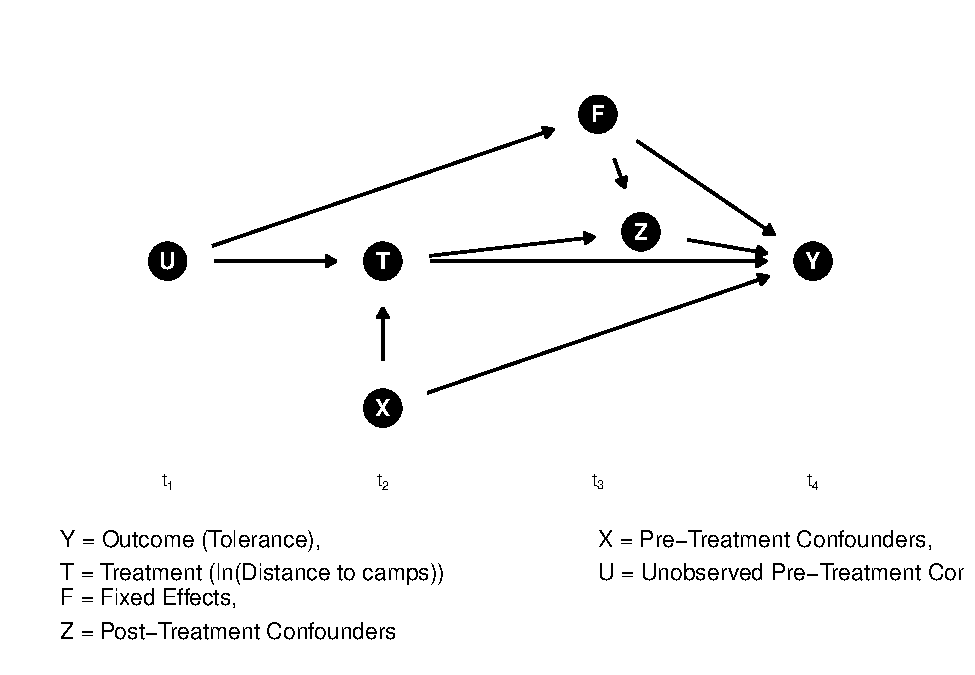
\includegraphics[width=0.85\linewidth]{tarea02_files/figure-latex/daghtp-1} \caption{DAG de la Figura 3 Pepinsky et al. (2024)}\label{fig:daghtp}
\end{figure}

Pepinsky et al. (\protect\hyperlink{ref-pepinsky_causation_2024}{2024}) refutan esto, argumentando que Homola et al. (\protect\hyperlink{ref-homola_fixed_2024}{2024}) no comprenden los errores de estimación. Sostienen que para que sus estimaciones con EF generen sesgo de pos-tratamiento, debe demostrarse que la distancia a los campos tiene un efecto causal en la formación de los Länder contemporáneos o sus características. Aunque esto no está respaldado por la evidencia presentada, Pepinsky et al. (\protect\hyperlink{ref-pepinsky_causation_2024}{2024}) asumen la estructura causal de Homola et al. (\protect\hyperlink{ref-homola_fixed_2024}{2024}), donde la distancia a los campos afecta variables pos-tratamiento \(Z\) (como el currículum escolar) que son descendientes de los EF para Länder (ver Figura \ref{fig:daghtp}). Pepinsky et al. (\protect\hyperlink{ref-pepinsky_causation_2024}{2024}) sostienen que, incluso con esta estructura, el efecto causal de \(T\) en \(Y\) es identificable solo con la inclusión de EF para los Estados, ya que esto controla la heterogeneidad no observada que confunde la relación causal. En este sentido, los EF actúan como bloqueadores de confusión del factor \(U\) que afecta tanto a \(T\) como a \(Y\) (\protect\hyperlink{ref-wysocki_statistical_2022}{Wysocki et al., 2022}).

La raíz de esta discusión es si la distancia a los campos es un antecesor causal de los EF para los Länder. Para Pepinsky et al. (\protect\hyperlink{ref-pepinsky_causation_2024}{2024}), la interpretación de Homola et al. (\protect\hyperlink{ref-homola_fixed_2024}{2024}) sobre los EF está errada, ya que confunden las características que varían entre Estados con aquellas que varían dentro de ellos. En el caso del currículum escolar, los EF no capturan su variación, ya que esta varía principalmente dentro de los Estados y no entre ellos. ``Homola et al.~han confundido la observación de que la proximidad a los campamentos afecta a los programas escolares individuales con la observación de que los Estados determinan los programas educativos estatales'' (\protect\hyperlink{ref-pepinsky_causation_2024}{Pepinsky et al., 2024, p. 3}). En consecuencia, Homola et al. (\protect\hyperlink{ref-homola_fixed_2024}{2024}) atribuyen variables pos-tratamiento, que pueden ser mecanismos explicativos de la relación causal, a atributos que varían entre Estados, fusionando el confundidor F con la variable pos-tratamiento \(Z\) en la Figura \ref{fig:daghtp}.

\hypertarget{pregunta-2}{%
\section{Pregunta 2}\label{pregunta-2}}

Tenemos por objetivo evaluar el efecto de la \texttt{intolerancia} en el \texttt{apoyo\ a\ partidos\ de\ extrema\ derecha}. Para ello, utilice la \texttt{distancia} a campos de concentración como instrumento. Específicamente, estime los siguientes estimands:

\begin{enumerate}
\def\labelenumi{\alph{enumi})}
\tightlist
\item
  ITTD sin covariables y ITTD controlando por efectos fijos para Länders.
\item
  ITT sin covariables y ITT controlando por efectos fijos para Länders.
\item
  CACE sin covariables y CACE controlando por efectos fijos para Länders.
\end{enumerate}

Reporte sus estimaciones en dos tablas de calidad: una para estimaciones sin covariables y otra con las estimaciones que controlan por FE para Länders.

\begin{table}[h!]
\begin{center}
\scalebox{1}{
\begin{tabular}{l c c c}
\toprule
 & \multicolumn{3}{c}{Modelos VI} \\
\cmidrule(lr){2-4}
 & $ITT_D$ & $ITT$ & $CACE$ \\
\midrule
Distancia al campo & $-0.009^{**}$ & $-0.001^{*}$ &           \\
                   & $(0.003)$     & $(0.001)$    &           \\
Intolerancia       &               &              & $0.154$   \\
                   &               &              & $(0.079)$ \\
\midrule
Länder FE          & No            & No           & No        \\
R$^2$              & $0.005$       & $0.002$      & $-0.206$  \\
Adj. R$^2$         & $0.005$       & $0.002$      & $-0.207$  \\
Num. obs.          & $2075$        & $2075$       & $2075$    \\
RMSE               & $0.685$       & $0.153$      & $0.168$   \\
\bottomrule
\multicolumn{4}{l}{\scriptsize{Nota: Errores estándares robustos entre paréntesis. $^{**}p<0.01$; $^{*}p<0.05$}}
\end{tabular}
}
\caption{\label{tab:table1} Modelos de VI sin efectos fijos para apoyo a partidos de extrema derecha en base a Pepinsky et al. (2023)}
\label{table:coefficients}
\end{center}
\end{table}

\begin{table}[h!]
\begin{center}
\scalebox{1}{
\begin{tabular}{l c c c}
\toprule
 & \multicolumn{3}{c}{Modelos VI} \\
\cmidrule(lr){2-4}
 & $ITT_D$ & $ITT$ & $CACE$ \\
\midrule
Distancia al campo & $0.004$   & $0.001$   &           \\
                   & $(0.004)$ & $(0.001)$ &           \\
Intolerancia       &           &           & $0.148$   \\
                   &           &           & $(0.307)$ \\
\midrule
Länder FE          & Sí        & Sí        & Sí        \\
R$^2$              & $0.039$   & $0.016$   & $-0.164$  \\
Adj. R$^2$         & $0.031$   & $0.009$   & $-0.173$  \\
Num. obs.          & $2075$    & $2075$    & $2075$    \\
RMSE               & $0.676$   & $0.153$   & $0.166$   \\
\bottomrule
\multicolumn{4}{l}{\scriptsize{Nota: Errores estándares robustos entre paréntesis. $^{**}p<0.01$; $^{*}p<0.05$}}
\end{tabular}
}
\caption{\label{tab:table2} Modelos de VI con efectos fijos para apoyo a partidos de extrema derecha en base a Pepinsky et al. (2023)}
\label{table:coefficients}
\end{center}
\end{table}

\hypertarget{pregunta-3}{%
\section{Pregunta 3}\label{pregunta-3}}

En relación con sus estimaciones en el ítem 2:

\begin{enumerate}
\def\labelenumi{\alph{enumi})}
\tightlist
\item
  Interprete sus estimaciones: ITTD , ITT, y CACE. Además, mencione quiénes serían los cumplidores.
\end{enumerate}

El estimador de variable instrumental (VI) es útil para lidiar con posibles sesgos de variable omitida (heterogeneidad no observada) que al estar correlacionada con nuestras covariables introducen fuentes de endogeneidad en la estimación. Este estimador también puede combinarse con métodos de datos de panel, como los efectos fijos, para estimar de forma consistente los parámetros cuando tenemos efectos inobservables y endogeneidad en una o más variables independientes que varían con el tiempo (\protect\hyperlink{ref-wooldridge_introductory_2009}{Wooldridge, 2009, p. 534}). Asumiendo una situación de incumplimiento de asignación al tratamiento, se realizó una estimación de VI para conocer la relación causal entre la intolerancia y el apoyo a partidos de extrema derecha, empleando la distancia a los campos de concentración como instrumento con los datos de Pepinksy et al. (\protect\hyperlink{ref-pepinsky_modeling_2023}{2023}). En las Tablas \ref{tab:table1} y \ref{tab:table2} se muestran los modelos de VI para apoyo a partidos de extrema derecha, distinguiendo entre el efecto causal de la asignación del tratamiento (\(ITT\)) y el efecto causal promedio para los que recibieron el tratamiento (\(CACE\)) y si se controla (o no) por efectos fijos para Länders.

\hypertarget{itt_d-e-itt}{%
\subsection{ITT\_D e ITT}\label{itt_d-e-itt}}

En cuanto al efecto de asignación del tratamiento (\(ITT_D\) e \(ITT\)):

\begin{itemize}
\item
  \(ITT_D\): En la Tabla \ref{tab:table1}, el modelo para \(ITT_D\) indica que el efecto de la distancia sobre la intolerancia es negativo y estadísticamente significativo con un 99\% de confianza (\(\beta\) = -0.009, SE = 0.003, p \textless{} 0.01). Sin embargo, este efecto deja de ser estadísticamente significativo en la Tabla \ref{tab:table2} al controlar por EF para Länders, además de que su signo cambia a positivo (\(\beta\) = 0.004, SE = 0.004, p \textgreater{} 0.05).
\item
  \(ITT\): Los resultados del modelo para \(ITT\) de la Tabla \ref{tab:table1} sugieren que existe una relación negativa de la distancia a los campos de concentración en el apoyo a partidos de extrema derecha (\(\beta\) = -0.001, SE = 0.001), siendo un efecto estadísticamente significativo al 95\% de confianza. Al controlar por EF para Länders en la Tabla \ref{tab:table2}, los resultados del \(ITT\) dejan de ser estadísticamente significativos aunque su dirección se mantiene.
\end{itemize}

\hypertarget{cace}{%
\subsection{CACE}\label{cace}}

Respecto al efecto promedio del tratamiento para aquellos que cumplen con la asignación del tratamiento según el instrumento (\(CACE\)), los resultados de los modelos de VI muestran que, aunque su efecto es positivo, no es estadísticamente significativo. En la Tabla \ref{tab:table1}, el modelo \(CACE\) sin EF sugiere que el efecto promedio de la intolerancia sobre el apoyo a partidos de extrema derecha para los cumplidores es igual 0.15, aunque este efecto no es estadísticamente significativo a un 95\% de confianza (SE = 0.079, p \textgreater{} 0.05). Al controlar por EF para Estados en modelo \(CACE\) de la Tabla \ref{tab:table2} los resultados siguen siendo los mismos (\(\beta\) = 0.148, SE = 0.307). Con todo, no se encuentra evidencia de que la intolerancia tenga un efecto causal sobre el apoyo a partidos de extrema derecha. En cualquier diseño de variables instrumentales, la subpoblación que toma (o no toma) el tratamiento debido a la variación en el instrumento se conoce como el conjunto de ``cumplidores''. En este estudio, los cumplidores serían aquellos cuya proximidad a los campos de concentración determina su nivel de intolerancia y, en consecuencia, su apoyo a partidos de extrema derecha.

\hypertarget{supuestos-de-vi-y-cace}{%
\subsection{Supuestos de VI y CACE:}\label{supuestos-de-vi-y-cace}}

Para que una variable \(Z\) sea un instrumento válido para el efecto causal del tratamiento en el resultado debe satisfacer una serie de supuestos, los cuales son similares a la estimación de \(CACE\) bajo incumplimiento (\protect\hyperlink{ref-wooldridge_introductory_2009}{Wooldridge, 2009}):

\textbf{Relevancia}: \(Z\) debe estar correlacionada con la variable endógena \(X\): \[Cor(Z,X) \neq 0\] Generalmente este supuesto se comprueba con una regresión lineal entre el instrumento y la variable independiente endógena (primera etapa). En este caso, el instrumento \(Z\) distancia a los campos de concentración se asocia significativamente con la variable endógena intolerancia cuando no se incluyen EF para Estados, lo que indica que este efecto depende en gran medida de las diferencias propias de los Estados, que son constantes en el tiempo. Por tanto, los resultados sugieren que la distancia no es un buen instrumento para la relación causal entre intolerancia y apoyo a partidos de extrema derecha.

\textbf{Exogeneidad}: \(Z\) no debe correlacionarse con el término de error \(U\) que captura la heterogeneidad no observada: \[Cor(Z,U) = 0\] Esto generalmente se asume mediante teoría, ya que no es posible de comprobar empíricamente. Sustantivamente, implica asumir que la distancia a los campos no se correlaciona con ningún otro factor no observado que pueda confundir la relación causal de interés.

\textbf{Restricción de Exclusión}: \(Z\) debe afectar \(Y\) (apoyo a partidos de extrema derecha) solo a través de \(X\) (intolerancia): \[Cor(Z,Y|X) = 0\] Esto significa que la distancia a los campos sólo puede afectar al apoyo a partidos de extrema derecha a través de la intolerancia.

\begin{enumerate}
\def\labelenumi{\alph{enumi})}
\setcounter{enumi}{1}
\tightlist
\item
  Discuta tres supuestos de sus estimaciones de CACEs, ¿son realistas? ¿se podría señalar que los CACEs estimados son creíbles?
\end{enumerate}

Para realizar una estimación \(CACE\) deben considerarse la evaluación y cumplimiento de, al menos, cinco supuestos: i) SUTVA, ii) restricción de exclusión, iii) asignación aleatoria del instrumento (\(Z\)), iv) efecto promedio del instrumento (\(Z\)) sobre el tratamiento (\(D\)) debe ser diferente de cero, y v) la relación entre el instrumento (\(Z\)) y la probabilidad de recibir el tratamiento (\(D\)) debe ser consistente (monotónica) para todas las unidades. En este ejercicio, evaluaré los primeros tres supuestos de \(CACE\).

\textbf{SUTVA (Stable Unit Treatment Value Assumption):} El cumplimiento de SUTVA implicaría que la distancia a los campos de concentración (\(Z\)) afecta de manera consistente la intolerancia (\(X\)) dentro de cada individuo, sin que haya interacciones o efectos cruzados entre individuos debido a variaciones en \(Z\). Esto significa que \(Z\) influiría de manera uniforme en la intolerancia de todos los individuos sin efectos indirectos entre ellos. Sin embargo, demostrar este supuesto puede ser complicado, ya que, como argumentan Pepinksy et al. (\protect\hyperlink{ref-pepinsky_modeling_2023}{2023}), la relación causal entre la distancia a los campos y la intolerancia podría estar confundida por una heterogeneidad espacial no observada asociada a características específicas de los Estados-Länders alemanes. Esto sugiere que las diferencias geográficas podrían interactuar con \(Z\) y \(X\) de maneras que comprometen la uniformidad del efecto de \(Z\) sobre \(X\) entre todos los individuos, lo cual podría plantear dudas sobre el cumplimiento de SUTVA.

\textbf{Asignación aleatoria de Z:} Este supuesto implica que \(Z\) (distancia a los campos de concentración) es asignado de manera aleatoria y no está correlacionado con otras características observadas o no observadas que podrían influir tanto en la intolerancia (\(X\)) como en el apoyo a partidos de extrema derecha (\(Y\)). Esto asegura que \(Z\) sea exógeno y no endógeno en relación con los individuos. En nuestro estudio, se garantiza que la distancia a los campos de concentración no está influenciada por características individuales que podrían determinar la presencia o ausencia de campos cercanos a los individuos. Además, es plausible sostener que la distribución de los campos de concentración entre los Länders es potencialmente aleatoria, ya que estos están presentes en algunos Länders y ausentes en otros (\protect\hyperlink{ref-pepinsky_modeling_2023}{Pepinsky et al., 2023})

\textbf{Restricción de Exclusión:} Este supuesto establece que la distancia a los campos (\(Z\)) solo puede afectar el apoyo a partidos de extrema derecha (\(Y\)) a través del mecanismo de la intolerancia (\(X\)), sin tener efectos directos no mediados por \(X\) en \(Y\). Es fundamental para asegurar que las estimaciones de \(CACE\) capturen de manera precisa el efecto causal de interés. Sin embargo, demostrar este supuesto tanto empírica como teóricamente presenta desafíos significativos, dado que pueden existir diversas variables, tanto observadas como no observadas después del tratamiento, que actúen como mediadores o confundidores en la relación causal de interés. Como muestran los resultados, al incluir efectos fijos (EF), la distancia a los campos deja de ser un buen instrumento para la intolerancia, lo cual cuestiona la validez del supuesto de restricción de exclusión.

\hypertarget{pregunta-4}{%
\section{Pregunta 4}\label{pregunta-4}}

Utilizando intolerance como variable resultado, estime los modelos 5 y 6 de Table 1 en Pepinsky et al. (\protect\hyperlink{ref-pepinsky_modeling_2023}{2023}). Específicamente:

\begin{enumerate}
\def\labelenumi{\alph{enumi})}
\tightlist
\item
  Reporte sus resultados en una tabla de calidad similar a la Table 1 del artículo bajo replicación. Use las covariables mencionadas arriba en esta pauta\footnote{Note que no debe incluir como variable independiente la población en 1925.}.
\end{enumerate}

\begin{table}[h!]
\begin{center}
\scalebox{0.9}{
\begin{tabular}{l c c}
\toprule
 & Modelo 5 & Modelo 6 \\
\midrule
Distancia al campo                & $-0.016^{**}$ & $0.006$       \\
                                  & $(0.003)$     & $(0.005)$     \\
\% Judíos (1925)                  & $-0.897$      & $5.924$       \\
                                  & $(1.341)$     & $(4.412)$     \\
\% Desempleo (1933)               & $2.411^{**}$  & $1.075$       \\
                                  & $(0.589)$     & $(0.744)$     \\
Participación partido nazi (1933) & $-0.156$      & $-0.717^{**}$ \\
                                  & $(0.213)$     & $(0.257)$     \\
\midrule
Länder FE                         & No            & Sí            \\
Método                            & G-est         & G-est         \\
Num. obs.                         & $1376.000$    & $1376.000$    \\
\bottomrule
\multicolumn{3}{l}{\scriptsize{Nota: Errores estándares entre paréntesis. $^{**}p<0.01$; $^{*}p<0.05$}}
\end{tabular}
}
\caption{\label{tab:table3} Replicación de modelos de efectos directos controlados Pepinsky et al. (2023)}
\label{table:coefficients}
\end{center}
\end{table}

\begin{enumerate}
\def\labelenumi{\alph{enumi})}
\setcounter{enumi}{1}
\tightlist
\item
  En base a la Table 1 de Pepinsky et al. (\protect\hyperlink{ref-pepinsky_modeling_2023}{2023}), discuta dos diferencias conceptuales entre el modelo (5) y el modelo (3).
\end{enumerate}

Por un lado, el Modelo 3 de la Tabla 1 de Pepinsky et al. (\protect\hyperlink{ref-pepinsky_modeling_2023}{2023, p. 7}) utiliza un estimador OLS combinado (pooled OLS), que combina todos los datos sin considerar los efectos específicos de cada unidad y asume independencia entre las observaciones. Este enfoque puede resultar en estimaciones sesgadas y menos eficientes debido a la heterogeneidad no observada entre los Estados, subestimando los errores estándar y proporcionando pruebas estadísticas con valores p muy bajos (\protect\hyperlink{ref-wooldridge_introductory_2009}{Wooldridge, 2009}). El OLS combinado no controla adecuadamente por la variabilidad entre unidades, lo que puede llevar a conclusiones erróneas sobre el efecto del tratamiento.

Por otro lado, el Modelo 5 emplea un estimador de efectos directos controlados (ACDE) mediante la estimación-g secuencial (\protect\hyperlink{ref-acharya_explaining_2016}{Acharya et al., 2016}). A diferencia del OLS combinado, este método no solo incluye los controles pretratamiento del Modelo 3, sino que también incorpora una serie de covariables intermedias (\(Zi\)) y mediadores (\(Mi\)) para identificar la relación causal entre la distancia a los campos y la intolerancia. El ACDE busca aislar el efecto directo del tratamiento en la variable de resultado, fijando el valor de los mediadores en un valor observado para todas las unidades, lo que permite lidiar con los confounders postratamiento que pueden sesgar la relación entre los mediadores y la intolerancia (\protect\hyperlink{ref-acharya_explaining_2016}{Acharya et al., 2016}).

Las estrategias de identificación de ambos modelos son sustantivamente diferentes en varios aspectos. En primer lugar, el OLS combinado no considera los efectos específicos de cada unidad, lo que puede llevar a la omisión de variabilidad importante entre las unidades y a estimaciones sesgadas, mientras que el ACDE controla explícitamente por mediadores y covariables intermedias, siendo más eficiente. En segundo lugar, el OLS combinado no lidia con el sesgo de postratamiento, mientras que el ACDE aborda explícitamente este sesgo al incluir mediadores y covariables intermedias en el estimands de dos etapas demediado, resultando en estimaciones más robustas y precisas.

Además, las estimaciones del OLS combinado pueden ser ineficientes y menos precisas debido a la omisión de heterogeneidad no observada y a la asunción de independencia entre observaciones. Por el contrario, el ACDE proporciona estimaciones más eficientes y precisas al considerar la variabilidad entre unidades y al controlar por confounders intermedios y mediadores, mejorando la identificación del efecto causal directo y la precisión de las inferencias estadísticas (\protect\hyperlink{ref-acharya_explaining_2016}{Acharya et al., 2016}).

\begin{enumerate}
\def\labelenumi{\alph{enumi})}
\setcounter{enumi}{2}
\tightlist
\item
  Utilizando como ejemplo sus estimaciones del modelo (6), explique las nociones de efecto directo controlado promedio (ACDE) y efecto directo natural promedio (ANDE).
\end{enumerate}

Siguiendo a Acharya et al. (\protect\hyperlink{ref-acharya_explaining_2016}{2016}), el efecto directo controlado promedio (ACDE) es un método de estimación de efectos directos ante la presencia de variables postratamiento que pueden confundir o mediar la identificación causal. El ACDE busca conocer el efecto directo del tratamiento en la variable resultado, controlando por variables pre y post tratamiento observadas y fijando el valor del mediador (\(M\)) en un valor observado para todas las unidades. Esto se realiza mediante una estimación de dos etapas: primero, se identifica el efecto causal del mediador (\(M\)) en la variable dependiente (\(Y\)), neutralizando esta ruta causal; luego, se estima el efecto controlado directo del tratamiento (\(T\)) en la variable de resultado (\(Y\)), manteniendo constante el mediador (\(M\)). Un supuesto clave para el ACDE es la independencia secuencial, que establece que no hay variables omitidas para la relación entre el tratamiento (\(T\)) y la variable resultado (\(Y\)), ni variables intermedias omitidas que confundan la relación entre el mediador (\(M\)) y el resultado (\(Y\)). Además, el supuesto de no interacciones intermedias es relevante, pero puede relajarse bajo ciertas condiciones (\protect\hyperlink{ref-acharya_explaining_2016}{Acharya et al., 2016, p. 520}).

Por su parte, el efecto directo natural promedio (ANDE) también es un método de estimación de efectos directos ante la presencia de variables postratamiento, pero incluye supuestos más fuertes para la identificación (\protect\hyperlink{ref-acharya_explaining_2016}{Acharya et al., 2016}). El ANDE busca conocer el efecto del tratamiento (\(T\)) en la variable resultado (\(Y\)) fijando el mediador (\(M\)) en un valor potencial-contrafactual del tratamiento. Según Acharya et al. (\protect\hyperlink{ref-acharya_explaining_2016}{2016, p. 516}), ``El efecto directo natural representa el efecto de un tratamiento modificado que no afecta al mediador, pero sigue afectando directamente al resultado''. Esto se logra mediante una formulación contrafactual de la relación causal que incluye el mediador, estimando el efecto del tratamiento en el resultado, dejando constante el mediador en el valor que hubiera tomado bajo la situación de control del tratamiento. Para que el ANDE sea identificable sin sesgo, se requieren supuestos más estrictos que el ACDE, especialmente en relación con la independencia secuencial, ya que no deben existir variables intermedias tanto observables (\(Z\)) como inobservables (\(U_2\)) que confundan la relación entre el mediador (\(M\)) y el resultado (\(Y\)) (\protect\hyperlink{ref-acharya_explaining_2016}{Acharya et al., 2016, p. 520}).

Las diferencias clave entre ACDE y ANDE residen en cómo se fija el mediador y el grado de rigidez del supuesto de independencia secuencial respecto a las variables intermedias observadas y no observadas. El Modelo 6 de la Tabla 3 muestra el ACDE de la distancia a los campos en la intolerancia, incluyendo covariables pretratamiento y efectos fijos para Länders. Los resultados de este modelo sugieren un efecto positivo aunque no estadísticamente significativo (B = 0.006, p \textgreater{} 0.05) de la distancia a los campos en la intolerancia, manteniendo los mediadores (\(M\)) fijos para todas las unidades. Si esta relación fuera estimada con un ANDE, no deberían existir covariables \(Z\) en la estimación, ni posibles variables omitidas a este nivel, lo cual es difícil de sostener, como argumentan Pepinsky et al. (\protect\hyperlink{ref-pepinsky_causation_2024}{2024}). Además, requeriría una formulación contrafactual para estimar la relación de la distancia (\(T\)) en la intolerancia (\(Y\)), dejando constantes los mediadores (\(M\)) en el valor que hubieran tomado bajo la situación de control de la distancia.

\hypertarget{pregunta-5}{%
\section{Pregunta 5}\label{pregunta-5}}

En nota al pie 2, Pepinsky et al. (\protect\hyperlink{ref-pepinsky_causation_2024}{2024}) sostienen:

\begin{quote}
Sequential g-estimation, which HPT propose as a solution because they believe that Länder fixed effects are post-treatment variables, is unnecessary. It is also probably biased, because sequential g-estimation also requires different assumptions that they neither acknowledge nor defend, and only identifies a specific causal effect of T under the assumption of sequential unconfoundedness (see \protect\hyperlink{ref-acharya_explaining_2016}{Acharya et al., 2016, p. 519}), which would require (among other things) that there are no unobserved confounders of the causal relationship between states and contemporary tolerance. Without that assumption, about which HPT are silent, sequential g-estimation does not resolve any identification problem.
\end{quote}

Al respecto, explique por qué la estimación-g secuencial que proponen Homola et al. (\protect\hyperlink{ref-homola_fixed_2024}{2024}) sería probablemente sesgada.

De acuerdo con Acharya et al. (\protect\hyperlink{ref-acharya_explaining_2016}{2016}), un problema asociado a la estimación de efectos directos, controlados o no, es el sesgo de variable intermedia, un tipo de sesgo de postratamiento. Este sesgo se refiere a variables intermedias (\(Z_i\)) tanto observadas como no observadas en la ruta causal de interés, es decir, variables afectadas por el tratamiento que a su vez influyen en el mediador y en la variable de resultado (p.~515). La lógica detrás de este sesgo es que condicionar por un mediador induce un sesgo de selección (M-bias), que afecta la estimación causal de interés (\protect\hyperlink{ref-wysocki_statistical_2022}{Wysocki et al., 2022}), a menos que todos los confounders intermedios \(Z_i\) sean incluidos, lo que puede resultar en un sesgo de postratamiento (\protect\hyperlink{ref-pepinsky_modeling_2023}{Pepinsky et al., 2023}).

Para lidiar con este problema de sesgo de variable intermedia, Acharya et al. (\protect\hyperlink{ref-acharya_explaining_2016}{2016}) proponen un método llamado estimación-g secuencial que, bajo ciertos supuestos, ha demostrado ser una estimación consistente para los efectos directos controlados (ACDE). A diferencia de otros enfoques como los efectos naturales, la estimación-g secuencial puede identificar el ACDE en presencia de confounders intermedios \(Z_i\). Sin embargo, para que esta estimación sea libre de sesgo, debe cumplirse al menos un supuesto clave en la identificación no paramétrica del ACDE, llamado independencia secuencia o ``sequential unconfoundedness''. Este supuesto implica que: i) no hay variables omitidas que afecten el efecto del tratamiento (\(Ti\)) en la variable de resultado (\(Yi\)) condicionadas por los confounders pretratamiento (\(Xi\)), y ii) no hay variables omitidas que afecten el efecto del mediador (\(Mi\)) en la variable de resultado (\(Yi\)) condicionadas por el tratamiento (\(Ti\)), los confounders pretratamiento (\(X_i\)) y los confounders intermedios (\(Zi\)). Esto significa que las rutas \(A_i\) ← \(U_{i1}\) → \(Yi\) y \(Mi\) ← \(U_{i2}\) → \(Yi\) no deben existir, asumiendo que se incluyen suficientes controles o covariables pretratamiento Xi e intermedias \(Z_i\) para bloquear estas rutas y evitar el sesgo de variable omitida (\protect\hyperlink{ref-acharya_explaining_2016}{Acharya et al., 2016}).

Si bien la primera parte del supuesto de sequential unconfoundedness es más plausible de corregir, la segunda no lo es tanto. El sesgo de variable omitida o de heterogeneidad no observada en estudios observacionales es difícil de combatir, ya que generalmente existen variables no observadas postratamiento que pueden confundir el efecto del mediador en la variable de resultado (\protect\hyperlink{ref-acharya_explaining_2016}{Acharya et al., 2016}). Precisamente, esto es lo que Pepinsky et al. (\protect\hyperlink{ref-pepinsky_causation_2024}{2024}) cuestionan en la estrategia de identificación de Homola et al. (\protect\hyperlink{ref-homola_fixed_2024}{2024}), al asumir que no existen confounders intermedios \(Z_i\) no observados que puedan afectar la estimación causal de la distancia a los campos en la intolerancia, lo cual es difícil de sostener.

\hypertarget{referencias}{%
\section{Referencias}\label{referencias}}

\hypertarget{refs}{}
\begin{CSLReferences}{1}{0}
\leavevmode\vadjust pre{\hypertarget{ref-acharya_explaining_2016}{}}%
Acharya, A., Blackwell, M., \& Sen, M. (2016). Explaining {Causal Findings Without Bias}: {Detecting} and {Assessing Direct Effects}. \emph{American Political Science Review}, \emph{110}(3), 512--529. \url{https://doi.org/10.1017/S0003055416000216}

\leavevmode\vadjust pre{\hypertarget{ref-homola_legacies_2020}{}}%
Homola, J., Pereira, M. M., \& Tavits, M. (2020). Legacies of the {Third Reich}: {Concentration Camps} and {Out-group Intolerance}. \emph{American Political Science Review}, \emph{114}(2), 573--590. \url{https://doi.org/10.1017/S0003055419000832}

\leavevmode\vadjust pre{\hypertarget{ref-homola_fixed_2024}{}}%
Homola, J., Pereira, M. M., \& Tavits, M. (2024). Fixed {Effects} and {Post-Treatment Bias} in {Legacy Studies}. \emph{American Political Science Review}, \emph{118}(1), 537--544. \url{https://doi.org/10.1017/S0003055423001351}

\leavevmode\vadjust pre{\hypertarget{ref-pearl_book_2018}{}}%
Pearl, J., \& Mackenzie, D. (2018). \emph{The book of why: The new science of cause and effect}. New York: Basic Books.

\leavevmode\vadjust pre{\hypertarget{ref-pepinsky_modeling_2023}{}}%
Pepinsky, T. B., Goodman, S. W., \& Ziller, C. (2023). Modeling {Spatial Heterogeneity} and {Historical Persistence}: {Nazi Concentration Camps} and {Contemporary Intolerance}. \emph{American Political Science Review}, \emph{118}(1), 519--528. \url{https://doi.org/10.1017/S0003055423000072}

\leavevmode\vadjust pre{\hypertarget{ref-pepinsky_causation_2024}{}}%
Pepinsky, T. B., Goodman, S. W., \& Ziller, C. (2024). Causation and {History} in {Legacy Studies}: {A Reply} to {Homola}, {Pereira}, and {Tavits}. \emph{SSRN Electronic Journal}. \url{https://doi.org/10.2139/ssrn.4705690}

\leavevmode\vadjust pre{\hypertarget{ref-wooldridge_introductory_2009}{}}%
Wooldridge, J. M. (2009). \emph{{Introductory econometrics: a modern approach}} (4th ed). Mason, OH: South Western, Cengage Learning.

\leavevmode\vadjust pre{\hypertarget{ref-wysocki_statistical_2022}{}}%
Wysocki, A. C., Lawson, K. M., \& Rhemtulla, M. (2022). Statistical {Control Requires Causal Justification}. \emph{Advances in Methods and Practices in Psychological Science}, \emph{5}(2), 25152459221095823. \url{https://doi.org/10.1177/25152459221095823}

\end{CSLReferences}

\pagebreak

\hypertarget{cuxf3digo-de-r}{%
\section{Código de R}\label{cuxf3digo-de-r}}

\begin{Shaded}
\begin{Highlighting}[]
\NormalTok{knitr}\SpecialCharTok{::}\NormalTok{opts\_chunk}\SpecialCharTok{$}\FunctionTok{set}\NormalTok{(}\AttributeTok{echo =}\NormalTok{ F,}
                      \AttributeTok{warning =}\NormalTok{ F,}
                      \AttributeTok{error =}\NormalTok{ F, }
                      \AttributeTok{message =}\NormalTok{ F) }
\ControlFlowTok{if}\NormalTok{ (}\SpecialCharTok{!} \FunctionTok{require}\NormalTok{(}\StringTok{"pacman"}\NormalTok{)) }\FunctionTok{install.packages}\NormalTok{(}\StringTok{"pacman"}\NormalTok{)}

\NormalTok{pacman}\SpecialCharTok{::}\FunctionTok{p\_load}\NormalTok{(tidyverse,}
\NormalTok{               rio,}
\NormalTok{               sjmisc,}
\NormalTok{               AER,}
\NormalTok{               sandwich,}
\NormalTok{               DirectEffects,}
\NormalTok{               estimatr,}
\NormalTok{               panelr,}
\NormalTok{               plm,}
\NormalTok{               clubSandwich,}
\NormalTok{               texreg,}
\NormalTok{               ggeffects)}

\FunctionTok{options}\NormalTok{(}\AttributeTok{scipen=}\DecValTok{999}\NormalTok{)}
\FunctionTok{rm}\NormalTok{(}\AttributeTok{list =} \FunctionTok{ls}\NormalTok{())}
\NormalTok{db\_or }\OtherTok{\textless{}{-}}\NormalTok{ rio}\SpecialCharTok{::}\FunctionTok{import}\NormalTok{(}\AttributeTok{file =} \StringTok{"../input/data/EVS\_main.csv"}\NormalTok{) }\SpecialCharTok{\%\textgreater{}\%} 
  \FunctionTok{as\_tibble}\NormalTok{()}


\NormalTok{miles }\OtherTok{\textless{}{-}} \ControlFlowTok{function}\NormalTok{(x) \{}
  \FunctionTok{format}\NormalTok{(}\FunctionTok{round}\NormalTok{(}\FunctionTok{as.numeric}\NormalTok{(x),}\DecValTok{0}\NormalTok{), }\AttributeTok{big.mark =} \StringTok{"."}\NormalTok{)}
\NormalTok{\}}

\NormalTok{decimales }\OtherTok{\textless{}{-}} \ControlFlowTok{function}\NormalTok{(x) \{}
  \FunctionTok{format}\NormalTok{(}\FunctionTok{round}\NormalTok{(}\FunctionTok{as.numeric}\NormalTok{(x), }\DecValTok{2}\NormalTok{), }\AttributeTok{decimal.mark =} \StringTok{","}\NormalTok{)}
\NormalTok{\}}

\NormalTok{custom\_extract }\OtherTok{\textless{}{-}} \ControlFlowTok{function}\NormalTok{(model) \{}
\NormalTok{  tr }\OtherTok{\textless{}{-}} \FunctionTok{extract}\NormalTok{(model)}
  
  \CommentTok{\# Identificar índices a conservar (excluyendo "R$\^{}2$", "s\_idios" y "s\_id")}
\NormalTok{  gof\_indices }\OtherTok{\textless{}{-}} \FunctionTok{which}\NormalTok{(}\SpecialCharTok{!}\NormalTok{(tr}\SpecialCharTok{@}\NormalTok{gof.names }\SpecialCharTok{\%in\%} \FunctionTok{c}\NormalTok{(}\StringTok{"R$\^{}2$"}\NormalTok{, }\StringTok{"s\_idios"}\NormalTok{, }\StringTok{"s\_id"}\NormalTok{)))}
  
  \CommentTok{\# Actualizar gof, gof.names y gof.decimal simultáneamente}
\NormalTok{  tr}\SpecialCharTok{@}\NormalTok{gof.names }\OtherTok{\textless{}{-}}\NormalTok{ tr}\SpecialCharTok{@}\NormalTok{gof.names[gof\_indices]}
\NormalTok{  tr}\SpecialCharTok{@}\NormalTok{gof }\OtherTok{\textless{}{-}}\NormalTok{ tr}\SpecialCharTok{@}\NormalTok{gof[gof\_indices]}
\NormalTok{  tr}\SpecialCharTok{@}\NormalTok{gof.decimal }\OtherTok{\textless{}{-}}\NormalTok{ tr}\SpecialCharTok{@}\NormalTok{gof.decimal[gof\_indices]}
  
  \FunctionTok{return}\NormalTok{(tr)}
\NormalTok{\}}
\CommentTok{\# set theme}

\FunctionTok{theme\_set}\NormalTok{(}\FunctionTok{theme\_bw}\NormalTok{())}


\FunctionTok{library}\NormalTok{(dagitty) }\CommentTok{\# Instalar V8}
\FunctionTok{library}\NormalTok{(ggdag)}

\NormalTok{coords }\OtherTok{\textless{}{-}} \FunctionTok{list}\NormalTok{(}
  \AttributeTok{x =} \FunctionTok{c}\NormalTok{(}\AttributeTok{Y=}\DecValTok{2}\NormalTok{, }\AttributeTok{T=}\DecValTok{0}\NormalTok{, }\AttributeTok{U=}\SpecialCharTok{{-}}\DecValTok{1}\NormalTok{, }\AttributeTok{F=}\DecValTok{1}\NormalTok{, }\AttributeTok{X=}\DecValTok{0}\NormalTok{, }\AttributeTok{T1=}\SpecialCharTok{{-}}\DecValTok{1}\NormalTok{, }\AttributeTok{T2=}\DecValTok{0}\NormalTok{, }\AttributeTok{Z=}\FloatTok{1.2}\NormalTok{),}
  \AttributeTok{y =} \FunctionTok{c}\NormalTok{(}\AttributeTok{Y=}\DecValTok{1}\NormalTok{, }\AttributeTok{T=}\DecValTok{1}\NormalTok{, }\AttributeTok{U=}\DecValTok{1}\NormalTok{, }\AttributeTok{F=}\DecValTok{2}\NormalTok{, }\AttributeTok{X=}\DecValTok{0}\NormalTok{, }\AttributeTok{T1=}\SpecialCharTok{{-}}\DecValTok{1}\NormalTok{, }\AttributeTok{T2=}\SpecialCharTok{{-}}\DecValTok{1}\NormalTok{, }\AttributeTok{Z=}\FloatTok{1.2}\NormalTok{)}
\NormalTok{  )}

\NormalTok{HPTbestcase }\OtherTok{\textless{}{-}} \FunctionTok{dagify}\NormalTok{(}
\NormalTok{  Y }\SpecialCharTok{\textasciitilde{}}\NormalTok{ T }\SpecialCharTok{+}\NormalTok{ F }\SpecialCharTok{+}\NormalTok{ X }\SpecialCharTok{+}\NormalTok{ Z,}
\NormalTok{  F }\SpecialCharTok{\textasciitilde{}}\NormalTok{ U,}
\NormalTok{  Z }\SpecialCharTok{\textasciitilde{}}\NormalTok{ T }\SpecialCharTok{+}\NormalTok{ F,}
\NormalTok{  T }\SpecialCharTok{\textasciitilde{}}\NormalTok{ U }\SpecialCharTok{+}\NormalTok{ X,}
  \AttributeTok{exposure =} \StringTok{"T"}\NormalTok{,}
  \AttributeTok{outcome =} \StringTok{"Y"}\NormalTok{,}
  \AttributeTok{coords =}\NormalTok{ coords}
\NormalTok{)}

\NormalTok{tidy\_dag }\OtherTok{\textless{}{-}} \FunctionTok{tidy\_dagitty}\NormalTok{(HPTbestcase)}

\NormalTok{tidy\_dag}\SpecialCharTok{$}\NormalTok{data}\SpecialCharTok{$}\NormalTok{time }\OtherTok{\textless{}{-}} \FunctionTok{c}\NormalTok{(}\StringTok{"t3"}\NormalTok{, }\StringTok{"t3"}\NormalTok{, }\StringTok{"t2"}\NormalTok{, }\StringTok{"t2"}\NormalTok{, }\StringTok{"t1"}\NormalTok{, }\StringTok{"t1"}\NormalTok{, }\StringTok{"t2"}\NormalTok{, }\StringTok{"t2"}\NormalTok{, }\StringTok{"t3"}\NormalTok{, }\StringTok{"t4"}\NormalTok{)}

\FunctionTok{ggdag}\NormalTok{(tidy\_dag, }\AttributeTok{node\_size=}\DecValTok{8}\NormalTok{, }\AttributeTok{text\_size =} \DecValTok{4}\NormalTok{) }\SpecialCharTok{+}
  \FunctionTok{theme\_classic}\NormalTok{() }\SpecialCharTok{+} \FunctionTok{remove\_axes}\NormalTok{() }\SpecialCharTok{+} \FunctionTok{theme}\NormalTok{(}\AttributeTok{axis.line=}\FunctionTok{element\_blank}\NormalTok{()) }\SpecialCharTok{+}
  \FunctionTok{ylim}\NormalTok{(}\SpecialCharTok{{-}}\FloatTok{1.5}\NormalTok{, }\FloatTok{2.5}\NormalTok{) }\SpecialCharTok{+} \FunctionTok{xlim}\NormalTok{(}\SpecialCharTok{{-}}\FloatTok{1.5}\NormalTok{,}\FloatTok{2.5}\NormalTok{) }\SpecialCharTok{+}
  \FunctionTok{geom\_text}\NormalTok{(}\AttributeTok{x=}\SpecialCharTok{{-}}\DecValTok{1}\NormalTok{, }\AttributeTok{y=}\SpecialCharTok{{-}}\NormalTok{.}\DecValTok{5}\NormalTok{, }\AttributeTok{label=}\FunctionTok{expression}\NormalTok{(t[}\DecValTok{1}\NormalTok{]), }\AttributeTok{size=}\DecValTok{3}\NormalTok{) }\SpecialCharTok{+}
  \FunctionTok{geom\_text}\NormalTok{(}\AttributeTok{x=}\DecValTok{0}\NormalTok{, }\AttributeTok{y=}\SpecialCharTok{{-}}\NormalTok{.}\DecValTok{5}\NormalTok{, }\AttributeTok{label=}\FunctionTok{expression}\NormalTok{(t[}\DecValTok{2}\NormalTok{]), }\AttributeTok{size=}\DecValTok{3}\NormalTok{) }\SpecialCharTok{+}
  \FunctionTok{geom\_text}\NormalTok{(}\AttributeTok{x=}\DecValTok{1}\NormalTok{, }\AttributeTok{y=}\SpecialCharTok{{-}}\NormalTok{.}\DecValTok{5}\NormalTok{, }\AttributeTok{label=}\FunctionTok{expression}\NormalTok{(t[}\DecValTok{3}\NormalTok{]), }\AttributeTok{size=}\DecValTok{3}\NormalTok{) }\SpecialCharTok{+}
  \FunctionTok{geom\_text}\NormalTok{(}\AttributeTok{x=}\DecValTok{2}\NormalTok{, }\AttributeTok{y=}\SpecialCharTok{{-}}\NormalTok{.}\DecValTok{5}\NormalTok{, }\AttributeTok{label=}\FunctionTok{expression}\NormalTok{(t[}\DecValTok{4}\NormalTok{]), }\AttributeTok{size=}\DecValTok{3}\NormalTok{) }\SpecialCharTok{+}
  \FunctionTok{geom\_text}\NormalTok{(}\AttributeTok{x=}\SpecialCharTok{{-}}\FloatTok{1.5}\NormalTok{, }\AttributeTok{y=}\SpecialCharTok{{-}}\DecValTok{1}\NormalTok{, }\AttributeTok{label=}\StringTok{"Y = Outcome (Tolerance),}
\StringTok{T = Treatment (ln(Distance to camps))"}\NormalTok{, }\AttributeTok{hjust=}\DecValTok{0}\NormalTok{) }\SpecialCharTok{+}
  \FunctionTok{geom\_text}\NormalTok{(}\AttributeTok{x=}\SpecialCharTok{{-}}\FloatTok{1.5}\NormalTok{, }\AttributeTok{y=}\SpecialCharTok{{-}}\FloatTok{1.4}\NormalTok{, }\AttributeTok{label=}\StringTok{"F = Fixed Effects,}
\StringTok{Z = Post{-}Treatment Confounders"}\NormalTok{, }\AttributeTok{hjust=}\DecValTok{0}\NormalTok{) }\SpecialCharTok{+}
  \FunctionTok{geom\_text}\NormalTok{(}\AttributeTok{x=}\DecValTok{1}\NormalTok{, }\AttributeTok{y=}\SpecialCharTok{{-}}\DecValTok{1}\NormalTok{, }\AttributeTok{label=}\StringTok{"X = Pre{-}Treatment Confounders,}
\StringTok{U = Unobserved Pre{-}Treatment Confounders"}\NormalTok{, }\AttributeTok{hjust=}\DecValTok{0}\NormalTok{)}
\CommentTok{\# Seleccionar: No}

\NormalTok{db }\OtherTok{\textless{}{-}}\NormalTok{ db\_or }\SpecialCharTok{\%\textgreater{}\%}
\NormalTok{  janitor}\SpecialCharTok{::}\FunctionTok{clean\_names}\NormalTok{()}

\CommentTok{\# Filtrar: No}

\CommentTok{\# Recodificar }
\NormalTok{sjmisc}\SpecialCharTok{::}\FunctionTok{frq}\NormalTok{(db}\SpecialCharTok{$}\NormalTok{state)}
\NormalTok{db}\SpecialCharTok{$}\NormalTok{state }\OtherTok{\textless{}{-}} \FunctionTok{as.factor}\NormalTok{(db}\SpecialCharTok{$}\NormalTok{state)}

\CommentTok{\# Tratamiento casos perdidos}
\FunctionTok{colSums}\NormalTok{(}\FunctionTok{is.na}\NormalTok{(db)) }\CommentTok{\# no NA}

\CommentTok{\# Transformar y derivar: No}

\CommentTok{\# ITT\_Y (Z {-}{-}\textgreater{} Y)}

\NormalTok{m1\_itt }\OtherTok{\textless{}{-}} \FunctionTok{lm\_robust}\NormalTok{(}\AttributeTok{formula =}\NormalTok{ far\_right }\SpecialCharTok{\textasciitilde{}}\NormalTok{ distance, }
                    \AttributeTok{se\_type =} \StringTok{"HC2"}\NormalTok{,}
                    \AttributeTok{data =}\NormalTok{ db)}
\NormalTok{m2\_itt }\OtherTok{\textless{}{-}} \FunctionTok{lm\_robust}\NormalTok{(}\AttributeTok{formula =}\NormalTok{ far\_right }\SpecialCharTok{\textasciitilde{}}\NormalTok{ distance, }
                    \AttributeTok{fixed\_effects =} \SpecialCharTok{\textasciitilde{}}\NormalTok{ state,}
                    \AttributeTok{se\_type =} \StringTok{"HC2"}\NormalTok{,}
                    \AttributeTok{data =}\NormalTok{ db)}

\CommentTok{\# IIT\_D (Z {-}{-}\textgreater{} D)}

\NormalTok{m1\_ittd }\OtherTok{\textless{}{-}} \FunctionTok{lm\_robust}\NormalTok{(}\AttributeTok{formula =}\NormalTok{ intolerance }\SpecialCharTok{\textasciitilde{}}\NormalTok{ distance, }
                     \AttributeTok{se\_type =} \StringTok{"HC2"}\NormalTok{,}
                     \AttributeTok{data =}\NormalTok{ db)}
\NormalTok{m2\_ittd }\OtherTok{\textless{}{-}} \FunctionTok{lm\_robust}\NormalTok{(}\AttributeTok{formula =}\NormalTok{ intolerance }\SpecialCharTok{\textasciitilde{}}\NormalTok{ distance, }
                     \AttributeTok{fixed\_effects =} \SpecialCharTok{\textasciitilde{}}\NormalTok{ state,}
                     \AttributeTok{se\_type =} \StringTok{"HC2"}\NormalTok{,}
                     \AttributeTok{data =}\NormalTok{ db)}

\CommentTok{\# CACE}

\NormalTok{m1\_iv }\OtherTok{\textless{}{-}} \FunctionTok{iv\_robust}\NormalTok{(}\AttributeTok{formula =}\NormalTok{ far\_right }\SpecialCharTok{\textasciitilde{}}\NormalTok{ intolerance }\SpecialCharTok{|}\NormalTok{ distance, }
                   \AttributeTok{se\_type =} \StringTok{"HC2"}\NormalTok{,}
                   \AttributeTok{data =}\NormalTok{ db, }
                   \AttributeTok{diagnostics =}\NormalTok{ T)}
\NormalTok{m2\_iv }\OtherTok{\textless{}{-}} \FunctionTok{iv\_robust}\NormalTok{(}\AttributeTok{formula =}\NormalTok{ far\_right }\SpecialCharTok{\textasciitilde{}}\NormalTok{ intolerance }\SpecialCharTok{|}\NormalTok{ distance,}
                   \AttributeTok{fixed\_effects =} \SpecialCharTok{\textasciitilde{}}\NormalTok{ state,}
                   \AttributeTok{se\_type =} \StringTok{"HC2"}\NormalTok{,}
                   \AttributeTok{data =}\NormalTok{ db,}
                   \AttributeTok{diagnostics =}\NormalTok{ T)}

\NormalTok{models1 }\OtherTok{\textless{}{-}} \FunctionTok{list}\NormalTok{(m1\_ittd, m1\_itt, m1\_iv)}
\NormalTok{models2 }\OtherTok{\textless{}{-}} \FunctionTok{list}\NormalTok{(m2\_ittd, m2\_itt, m2\_iv)}


\NormalTok{ccoef }\OtherTok{\textless{}{-}} \FunctionTok{list}\NormalTok{(}
  \AttributeTok{distance =} \StringTok{"Distancia al campo"}\NormalTok{,}
  \AttributeTok{intolerance =} \StringTok{"Intolerancia"}\NormalTok{)}

\NormalTok{texreg}\SpecialCharTok{::}\FunctionTok{texreg}\NormalTok{(}\AttributeTok{l =}\NormalTok{ models1,}
               \AttributeTok{include.ci =}\NormalTok{ F,}
               \AttributeTok{caption =} \FunctionTok{paste}\NormalTok{(}\StringTok{"(}\SpecialCharTok{\textbackslash{}\textbackslash{}}\StringTok{\#tab:table1)"}\NormalTok{,}\StringTok{"Modelos de VI sin efectos fijos para apoyo a partidos de extrema derecha en base a Pepinsky et al. (2023)"}\NormalTok{),}
               \AttributeTok{stars =} \FunctionTok{c}\NormalTok{(}\FloatTok{0.05}\NormalTok{, }\FloatTok{0.01}\NormalTok{),}
               \AttributeTok{custom.coef.map =}\NormalTok{ ccoef,}
               \AttributeTok{custom.note =} \StringTok{"Nota: Errores estándares robustos entre paréntesis. \%stars"}\NormalTok{,}
               \AttributeTok{custom.header =} \FunctionTok{list}\NormalTok{(}\StringTok{"Modelos VI"} \OtherTok{=} \DecValTok{1}\SpecialCharTok{:}\DecValTok{3}\NormalTok{),}
               \AttributeTok{custom.model.names =} \FunctionTok{c}\NormalTok{(}\StringTok{"$ITT\_D$"}\NormalTok{, }\StringTok{"$ITT$"}\NormalTok{, }\StringTok{"$CACE$"}\NormalTok{),}
               \AttributeTok{leading.zero =}\NormalTok{ T,}
               \AttributeTok{float.pos =} \StringTok{"h!"}\NormalTok{,}
               \AttributeTok{use.packages =}\NormalTok{ F,}
               \AttributeTok{booktabs =} \ConstantTok{TRUE}\NormalTok{,}
               \AttributeTok{scalebox =} \DecValTok{1}\NormalTok{,}
               \AttributeTok{digits =} \DecValTok{3}\NormalTok{,}
               \AttributeTok{custom.gof.rows =} \FunctionTok{list}\NormalTok{(}\StringTok{"Länder FE"} \OtherTok{=} \FunctionTok{c}\NormalTok{(}\StringTok{"No"}\NormalTok{, }\StringTok{"No"}\NormalTok{, }\StringTok{"No"}\NormalTok{)))}



\NormalTok{ccoef }\OtherTok{\textless{}{-}} \FunctionTok{list}\NormalTok{(}
  \AttributeTok{distance =} \StringTok{"Distancia al campo"}\NormalTok{,}
  \AttributeTok{intolerance =} \StringTok{"Intolerancia"}\NormalTok{)}

\NormalTok{texreg}\SpecialCharTok{::}\FunctionTok{texreg}\NormalTok{(}\AttributeTok{l =}\NormalTok{ models2,}
               \AttributeTok{include.ci =}\NormalTok{ F,}
               \AttributeTok{caption =} \FunctionTok{paste}\NormalTok{(}\StringTok{"(}\SpecialCharTok{\textbackslash{}\textbackslash{}}\StringTok{\#tab:table2)"}\NormalTok{,}\StringTok{"Modelos de VI con efectos fijos para apoyo a partidos de extrema derecha en base a Pepinsky et al. (2023)"}\NormalTok{),}
               \AttributeTok{stars =} \FunctionTok{c}\NormalTok{(}\FloatTok{0.05}\NormalTok{, }\FloatTok{0.01}\NormalTok{),}
               \AttributeTok{custom.coef.map =}\NormalTok{ ccoef,}
               \AttributeTok{custom.note =} \StringTok{"Nota: Errores estándares robustos entre paréntesis. \%stars"}\NormalTok{,}
               \AttributeTok{custom.header =} \FunctionTok{list}\NormalTok{(}\StringTok{"Modelos VI"} \OtherTok{=} \DecValTok{1}\SpecialCharTok{:}\DecValTok{3}\NormalTok{),}
               \AttributeTok{custom.model.names =} \FunctionTok{c}\NormalTok{(}\StringTok{"$ITT\_D$"}\NormalTok{, }\StringTok{"$ITT$"}\NormalTok{, }\StringTok{"$CACE$"}\NormalTok{),}
               \AttributeTok{leading.zero =}\NormalTok{ T,}
               \AttributeTok{float.pos =} \StringTok{"h!"}\NormalTok{,}
               \AttributeTok{use.packages =}\NormalTok{ F,}
               \AttributeTok{booktabs =} \ConstantTok{TRUE}\NormalTok{,}
               \AttributeTok{scalebox =} \DecValTok{1}\NormalTok{,}
               \AttributeTok{digits =} \DecValTok{3}\NormalTok{,}
               \AttributeTok{custom.gof.rows =} \FunctionTok{list}\NormalTok{(}\StringTok{"Länder FE"} \OtherTok{=} \FunctionTok{c}\NormalTok{(}\StringTok{"Sí"}\NormalTok{, }\StringTok{"Sí"}\NormalTok{, }\StringTok{"Sí"}\NormalTok{)))}



\NormalTok{m1\_direct }\OtherTok{\textless{}{-}} \FunctionTok{sequential\_g}\NormalTok{(}\AttributeTok{formula =}\NormalTok{ intolerance }\SpecialCharTok{\textasciitilde{}}\NormalTok{ distance }\SpecialCharTok{+} \CommentTok{\# A }
\NormalTok{                           prop\_jewish25 }\SpecialCharTok{+}  \CommentTok{\# X}
\NormalTok{                           unemployment33 }\SpecialCharTok{+} \CommentTok{\# X}
\NormalTok{                           nazishare33 }\SpecialCharTok{|}    \CommentTok{\# X}
\NormalTok{                           female }\SpecialCharTok{+}         \CommentTok{\# Z}
\NormalTok{                           age }\SpecialCharTok{+}            \CommentTok{\# Z }
\NormalTok{                           west }\SpecialCharTok{|}           \CommentTok{\# Z}
\NormalTok{                           lr }\SpecialCharTok{+}             \CommentTok{\# M}
\NormalTok{                           immigrants07 }\SpecialCharTok{+}   \CommentTok{\# M}
\NormalTok{                           unemployment07 }\SpecialCharTok{+} \CommentTok{\# M}
\NormalTok{                           unemp }\SpecialCharTok{+}          \CommentTok{\# M}
\NormalTok{                           educ }\SpecialCharTok{+}           \CommentTok{\# M}
\NormalTok{                           urban\_scale,     }\CommentTok{\# M}
                         \AttributeTok{data =}\NormalTok{ db)}

\NormalTok{m2\_direct }\OtherTok{\textless{}{-}} \FunctionTok{sequential\_g}\NormalTok{(}\AttributeTok{formula =}\NormalTok{ intolerance }\SpecialCharTok{\textasciitilde{}}\NormalTok{ distance }\SpecialCharTok{+} \CommentTok{\# A }
\NormalTok{                           prop\_jewish25 }\SpecialCharTok{+}  \CommentTok{\# X}
\NormalTok{                           unemployment33 }\SpecialCharTok{+} \CommentTok{\# X}
\NormalTok{                           nazishare33 }\SpecialCharTok{+}    \CommentTok{\# X}
\NormalTok{                           state }\SpecialCharTok{|}          \CommentTok{\# X (state fe as pre{-}treatment)}
\NormalTok{                           female }\SpecialCharTok{+}         \CommentTok{\# Z}
\NormalTok{                           age }\SpecialCharTok{+}            \CommentTok{\# Z }
\NormalTok{                           west }\SpecialCharTok{|}           \CommentTok{\# Z}
\NormalTok{                           lr }\SpecialCharTok{+}             \CommentTok{\# M}
\NormalTok{                           immigrants07 }\SpecialCharTok{+}   \CommentTok{\# M}
\NormalTok{                           unemployment07 }\SpecialCharTok{+} \CommentTok{\# M}
\NormalTok{                           unemp }\SpecialCharTok{+}          \CommentTok{\# M}
\NormalTok{                           educ }\SpecialCharTok{+}           \CommentTok{\# M}
\NormalTok{                           urban\_scale,     }\CommentTok{\# M}
                         \AttributeTok{data =}\NormalTok{ db)}


\CommentTok{\# extraer para tablas}

\NormalTok{summary\_m1\_direct }\OtherTok{\textless{}{-}} \FunctionTok{summary}\NormalTok{(m1\_direct)}
\NormalTok{coefnames }\OtherTok{\textless{}{-}} \FunctionTok{rownames}\NormalTok{(summary\_m1\_direct}\SpecialCharTok{$}\NormalTok{coefficients)}
\NormalTok{estimates }\OtherTok{\textless{}{-}}\NormalTok{ summary\_m1\_direct}\SpecialCharTok{$}\NormalTok{coefficients[, }\StringTok{"Estimate"}\NormalTok{]}
\NormalTok{stderrors }\OtherTok{\textless{}{-}}\NormalTok{ summary\_m1\_direct}\SpecialCharTok{$}\NormalTok{coefficients[, }\StringTok{"Std. Err."}\NormalTok{]}
\NormalTok{pvalues }\OtherTok{\textless{}{-}}\NormalTok{ summary\_m1\_direct}\SpecialCharTok{$}\NormalTok{coefficients[, }\StringTok{"Pr(\textgreater{}|t|)"}\NormalTok{]}
\NormalTok{n\_obs }\OtherTok{\textless{}{-}} \FunctionTok{as.integer}\NormalTok{(}\FunctionTok{length}\NormalTok{(m1\_direct}\SpecialCharTok{$}\NormalTok{fitted.values))}

\NormalTok{m1\_acde }\OtherTok{\textless{}{-}} \FunctionTok{createTexreg}\NormalTok{(}
  \AttributeTok{coef.names =}\NormalTok{ coefnames,}
  \AttributeTok{coef =}\NormalTok{ estimates,}
  \AttributeTok{se =}\NormalTok{ stderrors,}
  \AttributeTok{pvalues =}\NormalTok{ pvalues,}
  \AttributeTok{gof.names =} \FunctionTok{c}\NormalTok{(}\StringTok{"Num. obs."}\NormalTok{),}
  \AttributeTok{gof =} \FunctionTok{as.integer}\NormalTok{(}\FunctionTok{c}\NormalTok{(n\_obs))}
\NormalTok{)}

\NormalTok{summary\_m2\_direct }\OtherTok{\textless{}{-}} \FunctionTok{summary}\NormalTok{(m2\_direct)}
\NormalTok{coefnames }\OtherTok{\textless{}{-}} \FunctionTok{rownames}\NormalTok{(summary\_m2\_direct}\SpecialCharTok{$}\NormalTok{coefficients)}
\NormalTok{estimates }\OtherTok{\textless{}{-}}\NormalTok{ summary\_m2\_direct}\SpecialCharTok{$}\NormalTok{coefficients[, }\StringTok{"Estimate"}\NormalTok{]}
\NormalTok{stderrors }\OtherTok{\textless{}{-}}\NormalTok{ summary\_m2\_direct}\SpecialCharTok{$}\NormalTok{coefficients[, }\StringTok{"Std. Err."}\NormalTok{]}
\NormalTok{pvalues }\OtherTok{\textless{}{-}}\NormalTok{ summary\_m2\_direct}\SpecialCharTok{$}\NormalTok{coefficients[, }\StringTok{"Pr(\textgreater{}|t|)"}\NormalTok{]}
\NormalTok{n\_obs }\OtherTok{\textless{}{-}} \FunctionTok{as.integer}\NormalTok{(}\FunctionTok{length}\NormalTok{(m2\_direct}\SpecialCharTok{$}\NormalTok{fitted.values))}

\NormalTok{m2\_acde }\OtherTok{\textless{}{-}} \FunctionTok{createTexreg}\NormalTok{(}
  \AttributeTok{coef.names =}\NormalTok{ coefnames,}
  \AttributeTok{coef =}\NormalTok{ estimates,}
  \AttributeTok{se =}\NormalTok{ stderrors,}
  \AttributeTok{pvalues =}\NormalTok{ pvalues,}
  \AttributeTok{gof.names =} \FunctionTok{c}\NormalTok{(}\StringTok{"Num. obs."}\NormalTok{),}
  \AttributeTok{gof =} \FunctionTok{as.integer}\NormalTok{(}\FunctionTok{c}\NormalTok{(n\_obs))}
\NormalTok{)}


\NormalTok{ccoef }\OtherTok{\textless{}{-}} \FunctionTok{list}\NormalTok{(}
  \AttributeTok{distance =} \StringTok{"Distancia al campo"}\NormalTok{,}
  \AttributeTok{prop\_jewish25 =} \StringTok{"\% Judíos (1925)"}\NormalTok{,}
  \AttributeTok{unemployment33 =} \StringTok{"\% Desempleo (1933)"}\NormalTok{,}
  \AttributeTok{nazishare33 =} \StringTok{"Participación partido nazi (1933)"}
\NormalTok{  )}

\NormalTok{texreg}\SpecialCharTok{::}\FunctionTok{texreg}\NormalTok{(}\AttributeTok{l =} \FunctionTok{list}\NormalTok{(m1\_acde, m2\_acde),}
               \AttributeTok{caption =} \FunctionTok{paste}\NormalTok{(}\StringTok{"(}\SpecialCharTok{\textbackslash{}\textbackslash{}}\StringTok{\#tab:table3)"}\NormalTok{,}\StringTok{"Replicación de modelos de efectos directos controlados Pepinsky et al. (2023)"}\NormalTok{),}
               \AttributeTok{stars =} \FunctionTok{c}\NormalTok{(}\FloatTok{0.05}\NormalTok{, }\FloatTok{0.01}\NormalTok{),}
               \AttributeTok{custom.note =} \StringTok{"Nota: Errores estándares entre paréntesis. \%stars"}\NormalTok{,}
               \AttributeTok{custom.model.names =} \FunctionTok{c}\NormalTok{(}\StringTok{"Modelo 5"}\NormalTok{, }\StringTok{"Modelo 6"}\NormalTok{),}
               \AttributeTok{custom.coef.map =}\NormalTok{ ccoef,}
               \AttributeTok{leading.zero =}\NormalTok{ T,}
               \AttributeTok{float.pos =} \StringTok{"h!"}\NormalTok{,}
               \AttributeTok{use.packages =}\NormalTok{ F,}
               \AttributeTok{booktabs =} \ConstantTok{TRUE}\NormalTok{,}
               \AttributeTok{scalebox =} \FloatTok{0.90}\NormalTok{,}
               \AttributeTok{digits =} \DecValTok{3}\NormalTok{,}
               \AttributeTok{custom.gof.rows =} \FunctionTok{list}\NormalTok{(}\StringTok{"Länder FE"} \OtherTok{=} \FunctionTok{c}\NormalTok{(}\StringTok{"No"}\NormalTok{, }\StringTok{"Sí"}\NormalTok{),}
                                      \StringTok{"Método"} \OtherTok{=} \FunctionTok{rep}\NormalTok{(}\StringTok{"G{-}est"}\NormalTok{, }\DecValTok{2}\NormalTok{)))}
\end{Highlighting}
\end{Shaded}


\end{document}
